\documentclass[conference]{IEEEtran}

\usepackage[pdftex]{graphicx}
\usepackage[cmex10]{amsmath}
\usepackage{algorithmic}
\usepackage{caption}
\usepackage{subfig}
\usepackage{url}
\usepackage{balance}

\begin{document}
\title{What Can Stack Traces Tell us about of the use Exceptions in Java?}

\author{\IEEEauthorblockN{Roberta Coelho\IEEEauthorrefmark{1},
Georgios Gousios\IEEEauthorrefmark{2}, Arie van Deursen\IEEEauthorrefmark{2},
Lucas Almeida\IEEEauthorrefmark{1}}
\IEEEauthorblockA{\IEEEauthorrefmark{1}Federal University of Rio Grande do Norte\\
Natal, Brazil\\
Email: \texttt{roberta@dimap.ufrn.br,lucas.almeida@ppgsc.ufrn.br}}
\IEEEauthorblockA{\IEEEauthorrefmark{2}Delft University of Technology\\
Delft, The Netherlands\\
Email: \texttt{\{g.gousios,arie.vandeursen\}@tudelft.nl}}
}

\newcommand{\todo}[1]{\textbf{TODO}\footnote{\textbf{TODO:} #1}}

% make the title area
\maketitle

\begin{abstract}

In this work, we perform the first large scale analysis of Java stack traces and
pinpoint how they can reveal bad programming practices. We mined and analyzed
the stack traces embedded in all issues of Java projects available GitHub.
Overall, our research set includes 356,057 issues defined at 16,836 projects, 
from which 28,800 stack traces were extracted. From this set, the stack traces
of 482 Android projects were investigated in more detail, in combination with
source code and bytecode analysis. In this study some patterns of exception
(mis)-use were consistently detected such as: unexpected wrappings (e.g., Errors
being wrapped in checked exceptions), revealing that Java hybrid exception
model is not fully used according to its purpose;  undocumented runtime
exceptions signaled by third party code, which is a serious threat to program
dependability; and a high prevalence of java.lang exceptions reported on issues,  
they were found in aproximately 50\% of all analyzed exception stack traces.


\end{abstract}

%\IEEEpeerreviewmaketitle

\section{Introduction}

\subsection{Georgios's and Roberta's Merged Introduction}

Modern applications have to cope with an increasing number of abnormal
computation states that arise as a consequence of faults in the application
itself (e.g., access of null references), noisy user inputs or faults in
underlying middleware or hardware. The exception handling
mechanism~\cite{goodenough1975exception} is one of the most used schemes for
detecting and recovering from such exceptional conditions. When an exception is thrown it can be caught inside the application (by the program's exception handling code) and the the application has the opportunity to assess the conditions that caused the fault and either recover from them or abort. 
If the exception that remains uncaught (is not caught by an exception handler) it
leads to a program crash -  uncaught exceptions ~\cite{jo2004uncaught} are one 
of the main causes of application crashes.

 In most programming languages with embedded exception handling mechanism, when a crash happens usually the language runtime generates debugging information to help
the programmer identify and fix the cause of the crash. The debugging
information is typical a stack trace, which includes an explanatory message and
the execution stack frame when the exception occurred. In Java, stack trace
consists of an ordered list of methods that were active on the call stack before
the exception occurred.

Although the exception handling mechanism has been the target of several studies
(e.g.~\cite{miller1997issues,Robil00,shah2010understanding,
garcia2007extracting,garcia2001comparative,cabral2007exception,coelho2011unveiling}),
the exception handling code is often generally poorly understood and the least
tested part of software systems~\cite{coelho2011unveiling}. 

%Similarily to source
%code, 
%TODO GEORGIOUS I DID NOT UNDERESTA.ND THE IDEA OF THE PREVIOUS SENTENCE

Such studies  perform the analysis of exception handling code based  either on static
(source code-based) analysis or dynamic (runtime-based) testing methods. Neither of such methods, however,
can explore the full execution space of a program and therefore they both fail
to account for exceptions implicitly signaled by rutime environment (e.g. resource depletion) or
dynamically loaded code. Exception stack traces, when available, enable the
post-mortem analysis of exception handling behaviours of programs and
concequently the evaluation of exception handling mechanisms in programming
languages.

The availability of exception stack traces until recently was scarce, while the
available data were only focused on few large scale projects.
Along the recent years we have witnessed a rapid increase in the number of open source 
projects that make their control version and issue tracking systems publicly 
available in repository hosting sites such as GitHub.

The concentration of open source projects and the existence of
initiatives that mine such information, such as GHTorrent~\cite{Gousi13},
 allow the information about projects to be visible within and across projects and
 make a full population studies possible.

In this work, we perform the first post mortem analysis of exception handling in
Java.  Using a custom tool called ExceptionMiner, which we develop specifically
for this study, we mine stack traces from issues across all Java projects on
GitHub. Overall, we analyzed 356,057 issues from 16,836 projects, from which
28,800 stack traces were extracted and used as a source of information for our
analysis. The stack trace analysis was augmented by additional information
extracted using byte code and source code analysis done on a carefully selected
subset of our initial sample (482 Android projects). Manual inspection was also 
used in this study to leverage the understanding of stack traces and support 
further discussions and insights. 

To guide this exploration we compiled general 
guidelines on how to use exceptions proposed by Gosling~\cite{gosling2000java},
Wirfs-Brock~\cite{wirfs2006toward} and Bloch~\cite{bloch2008effective} and then
we investigate what stack traces can tell us about the adherence to such
practices in Java programs. Some outcomes were consistently detected through
our large scale analysis of exception stack traces in the wild, such as:

\begin{itemize}

   \item  A multitude of programming mistakes were reported as the main causes of stack traces:
  41,1\%  (12,625)  of reported stack traces were caused by programming mistakes; and 26,31\% of analyzed stack traces reported a java.lang.NullPointerException as root cause; 

   \item 1,671 projects (44,47\%) contained at least one issue reporting a java.lang.NullPointerException as the root cause of a stack trace.
   
  \item Undocumented runtime exceptions signaled by third party
    code (i.e., libraries and Android platform). This study found 118 distinct methods defined on third party code and  reported as the root signalers of runtime exceptions. Only 1 of such methods (0,8\%) documented the explicitly thrown runtime exception in a Javadoc comment; and none of these methods included the exception as part of the exception interface (i.e., using throws clause).

  \item  Odd exception chains (e.g., Error wrapping checked and runtime
    exceptions and vice-versa), indicating that the purpose of Java's hybrid
    exception model may not have been adequately used.

  \item  Issues reporting uncaught checked exceptions.


\end{itemize}

The contributions of this study are as follows:
\begin{itemize}

  \item  It performs the first large scale analysis of Java stack traces and how
    they can reveal bad-practices on the use of exceptions in Java.

  \item  It introduces ExceptionMiner, a tool developed to support cross-repository stack trace
    analysis.

\end{itemize}

These contributions are relevant to:
(i) developers of Java applications
to familiarize with the most common reported exceptions mis-uses which is the
first step to help developers to avoid making them;
(ii) designers of languages
to consider ways of reducing the abundance of NullPointerExceptions;
and (iii)
tool designers to consider developing tools that enable a cross-project defect
analysis.

% AVD: We have not looked at private issues, and the tool is described above.
%We strongly believe that, specially in the open-source environment,
%faults are not to be hidden in a private bug issue. Faults should be shared and
%discussed, so that a developer can learn from other projects mistakes.
%Currently, the search facilities of repositories are very limited, and the
%ExceptionMiner tool is a contribution in this direction.

%This paper is organized as follows. Section 2 presents a
%background on exception handling mechanism. Section 3 presents the study design.
%Section 4 reports study findings. Section 5 provides further discussions and insights.
%Section 6 presents the threats to validity associated to this study. Finally Section
%7 describes the related work, and Section 8 presents our conclusions and
%directions for future work.



\section{Background}

\subsection{Error Handling in Programming Languages}

Techniques for error detection and handling are not  an optional add-on but a
fundamental part of any system~\cite{bruntink2006discovering}. Several
approaches exist for detecting errors and responding to them, such as the return-code 
idiom (widely used in systems written in C), and the exception handling 
mechanism, embedded in many main-stream programming languages.
The main disadvantage of return codes is the fact that the programmer can just
ignore the return code and let the program execute in inconsistent state. 
The exception mechanism~\cite{goodenough1975exception} was proposed as a way of
preventing errors from being ignored and was embedded in many mainstream
programming languages ~\cite{garcia2001comparative} since then. 

In languages such as CLU\footnote{In CLU,  if a handler is 
found for a given exception, it is converted in a predened default exception, 
called failure which is the only one which can be implicitly 
propagated in this model [ref-clue].}, Modula-3, Guide, and Extended Ada the exceptions are 
checked, which means that the 
compiler statically checks if appropriate handlers are provided within the system. 
Accordingly, the programmer must explicitly specify every exception that can be
signaled to support the compile time checking. This approach is known to be
costly to maintain (Dooren and Steegmans, 2005) since exception updates are
cascading; if a new exception type is added to a method signature then all other
methods directly using this method must either change their signatures to
include the new exception type or handle the new exception. 

In languages such as Lore, C++, and Arche all exceptions are unchecked but the developer can optionally list exception types on method signatures. Although exceptions can 
be documented on methods signatures, the developer is not warned by the compiler
if an unchecked exception is not handled inside the application. According to ~\cite{Robil00} 
such an approach may hinder robustness because the client of a method cannot easily know
which unchecked exceptions may be thrown (unless the code of the method and the
methods called from it is inspected) which can be a very time consuming or
infeasible task. 

In Java a method can throw either checked or unchecked exceptions. Java is the only language that allows a hybrid approach on which the developer can define exceptions of both kinds to be thrown and handled in a single system. Next section details Java exception handling model.

Although exception handling mechanism is the most used technique to deal with such 
failures - been embedded in several programming languages as show above,   
the exception handling code is often generally poorly understood and the least
tested part of software systems.This behaviour may lead to the problem of uncaught exceptions~\cite{jo2004uncaught}, one of the main causes of application crashes
(e.g.~\cite{miller1997issues,Robil00,shah2010understanding, garcia2007extracting, garcia2001comparative,cabral2007exception,coelho2011unveiling}).


\subsection{Checked an Unchecked Exceptions in Java} \label{sec:extypes}

In Java, an exception is represented according to the class hierarchy shown in
Figure~\ref{fig:exchier}.  According to it every exception is an
instance of the Throwable class, and can be of three kinds: checked exceptions
(extends Exception), run-time exceptions (extends RuntimeException), and errors
(extends Error)~\cite{gosling2000java}.

\begin{figure} \centering 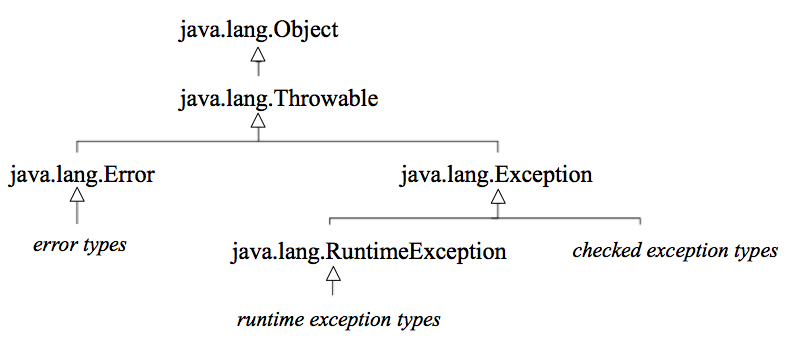
\includegraphics[width=\hsize]{new2_hierarchy.png}
  \caption{Exception Hierarchy in Java} \label{fig:exchier} \end{figure}

Neither run-time exceptions nor errors need to be specified on method
signatures, and hence both are referred as unchecked exceptions. The Java
Virtual Machine represents as runtime exceptions invalid operations detected in
the program (out-of-bounds array index, divide-by-zero error, null pointer
references) from which most of the programs are not expected to recover. By
convention an Error represents an unrecoverable condition which usually results
from failures detected by the Java Virtual Machine, such as OutOfMemoryError and
normally should not be handled inside the application.

The Java specification~\cite{gosling2000java} suggests that user-defined
exceptions should be checked exceptions. The main reason is because doing so the
callers of a method will know about the exceptions that a method can throw, and
so they can decide what to do about them. However, there is a long-lasting
debate about the use of checked and unchecked exceptions in
Java~\cite{javatut,stackoverlow,debate},\footnote{152 questions in Stackoverlow
are related to this debate} since there are pros and cons associated to each of
them.

Hence, in Java an exception can be thrown in one of the following
circumstances~\cite{gosling2000java}: (i) explicitly thrown when a throw statement is executed; 
(ii) implicitly thrown by the JVM when the evaluation of an expression
 violates the normal semantics of language (e.g., out-of-bounds array index,
division-by-zero, access to a null reference); or (iii) implicitly thrown by
the JVM due to an internal error or resource limitation (e.g.,
OutofMemoryError). 

%\todo{This sub-section is quite similar to the section introduction, shouldn't
%we merge them?}

When an exception is throw it causes a transfer of control from the point
where the exception occurred to a point that can be specified by the programmer
(exception handler) - in Java it is represented by the try-catch block .

A common way of  propagating exceptions in Java programs, is the exception wrapping (also known as exception chaining), which allows one exception to be wrapped in another exception and re-thrown. 
Figure~\ref{fig:wrapping} presents a stack trace associated which illustrates an
exception wrapping. The bottom part of the stack trace is the \emph{root cause}, which indicates the
first reason for the error to be thrown (in this case, the computer run out of
memory). The top part of the stack trace indicates the location of the exception
manifestation (which will call \emph{top level exception} along this paper). The
execution flow  between the root cause and the exception manifestation may
include other intermediate exception wrappings. In all levels, the exception
\emph{signaler}, is the method that threw the exception, represented on the
stack trace as the first method call below the exception declaration.

\begin{figure} \centering 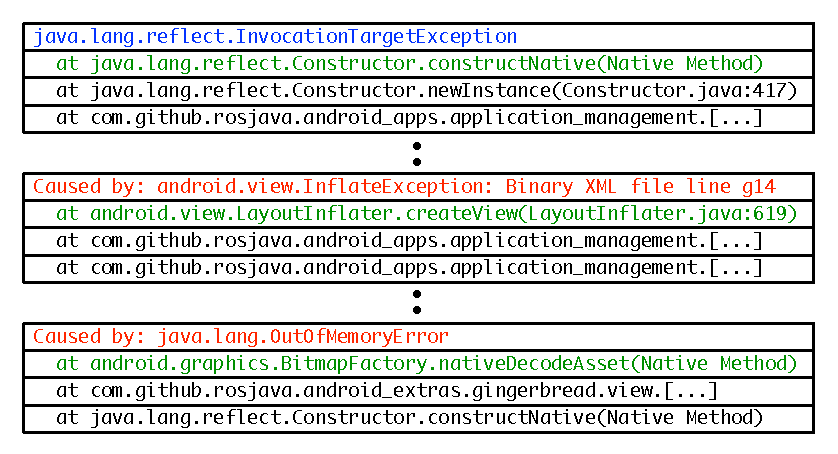
\includegraphics[scale=0.6]{wrappings}
\caption{Example of an Exception stack trace in Java.}
\label{fig:wrapping}
\end{figure}

\subsection{Exception Handling Best Practices in Java}
\label{sec:best}

Several general guidelines have been proposed on how to use Java
exceptions~\cite{mandrioli1992advances,gosling2000java,wirfs2006toward,
bloch2008effective}. 
A list of the guidelines related to exception types and exception
propagation in Java the following:\footnote{We also compiled guidelines related
to exception handling but they are out of the scope of this paper.}

%\noindent\emph{Meaning of Exception Types}

\textbf{I-Use checked exceptions to represent recoverable
conditions} (\cite{mandrioli1992advances,gosling2000java,wirfs2006toward,bloch2008effective})
The developer should use checked exceptions for conditions from which the caller
is expected to recover. By confronting the API user with a checked exception,
the API designer is forcing the client to handle the exceptional condition. The
client can explicitly ignore the exception (swallowing, or converting it to
other type) at the expense of the program's robustness~\cite{gosling2000java}.

\textbf{II-Error represents an unrecoverable condition detected by the JVM which
should not he handled} (\cite{gosling2000java}). It results from failures detected
by the Java Virtual Machine which indicate resource deficiencies, invariant
failures or other conditions that make impossible the program to recover.

%\noindent\emph{Exception Throwing}

\textbf{III-A method should throw exceptions that precisely define the
exceptional condition} (\cite{gosling2000java,bloch2008effective}). To do so,
developers should either try to reuse the exception types already defined in the
JVM or they should create a specific exception. Throwing general types such as a
pure Exception or a RuntimeException is hence considered a bad practice.

%\textbf{IV-Do not repeatedly re-throw exceptions, handle exceptions as close as
%possible to the problem}~\cite{wirfs2006toward}. 
%Programs that frequently throw exceptions lose in performance ~\cite{wirfs2006toward,gosling2000java}.
%Moreover, 
%Close to the place that the exception was throw the caller usually has
%enough contextual information to perform  corrective actions. When the exception
%is propagated far away from the method where it was signaled (i.e. further away
%#from the problem) it can be difficult to take meaningful recovery actions.
%*~\todo{RSC:this practice was not well explored, can be removed if we need space.}

%\noindent\emph{Exception Documentation}
\textbf{ IV-Document all exceptions thrown by a
method} (\cite{mandrioli1992advances,gosling2000java,wirfs2006toward,bloch2008effective}).
The exceptions thrown by a method are an important part of methods interface,
and is required to use the method properly. The checked exceptions are already
part of the  methods signature, and the method caller is aware of the checked
exceptions being thrown by it. According to~\cite{bloch2008effective}, it is
also wise to document the explicitly thrown runtime exceptions\footnote{This
excludes the implicitly signaled JVM runtime exceptions related to programming
mistakes} as carefully as checked exceptions. Doing so, the clients of a method
will be aware of all the exceptions the method can throw. If the developer fails to
do follow this practice (specially when developing library code) it will be
difficult or even impossible for the caller to make effective use of such 
method~\cite{wirfs2006toward, bloch2008effective}. As mentioned in Section II, 
in some languages such as C

These best practices guided our exploratory study described next.
Based on information extracted from stack traces (complemented by
bytecode and source-code analysis), we investigate whether stack characteristics
can reveal whether these practices have been obeyed. 
%Next section discusses the
%study procedure and the practices' misuses that emerged from this study.

\section{Study Design}

This work describes an exploratory study which was based on a sequential
mixed-methods approach~\cite{ivankova2006using} for collecting, analyzing, and
integrating both quantitative and qualitative evidence along the stages of the
research process. 

The main goal of this study was to gain a better understanding
of the use of exceptions in Java programs based mainly on the information
available on exception stack traces embedded on Github issues.
The exceptions available on exception stack trace are not limited to the exceptions 
expliciltly thrown by the Java developer but also include
the exceptions implicitly thrown by the JVM during the program execution,
due to a programming error (e.g., out-of-bounds array index, division-by-zero, 
access to a null reference) or an internal error or resource limitation (e.g.,
OutofMemoryError). 

 More specifically, we aimed at answering
the following research questions:

\begin{description}

  \item[RQ1] What are the common characteristics of such stack traces?

  \item[RQ2] What patterns of exception (mis)-use emerge from the stack trace
    analysis?

\end{description}

For RQ1 and RQ2, we explore the domain quantitatively and highlight interesting cases by 
exploring cases qualitatively. To support this investigation, source code and bytecode 
analysis were used in combination with manual inspection to leverage the  understanding of stack traces and support further discussions and insights. 

\subsection{Github Data}
\label{sec:git}

As mentioned before, this study amined at mining information available on GitHub issues,
more specifically, extracting and distilling the stack traces embedded on GItHub issues. 
Issues on Github are different from issues on dedicated bug tracking tools such as 
Bugzilla and Jira. The most important difference is that there are no predefined fields
  (e.g. severity and priority). Instead, Github uses a more open ended tagging system, on which
repositories are offered a pre-defined set of labels, but repository owners can modify 
them at will. Therefore, an issue may have none ore an arbitrary set of labels depending 
on which repository it was created. Therefore, this study is based on the assumption 
if an stack trace information embedded in an issue, it contain relevant information
 concerning the exception use -  regardless the lables associated to the issue.

Moreover, issues and pull requests are dual on Github; all pull requests have a corresponding 
``backing'' issue which
are automatically generated. Therefore, we excluded such automatically generated
issues from our analysis. Finally, the Github API allows the automated
generation of issues for specific repositories, which automated tools often use
to report crashes. In some cases, this led to high number of issues that
included stack traces. We identified and filtered those cases out (e.g.,
the~\textsf{pullwifi} project was responsible for almost 50\% of all Android issues in our dataset).

\subsubsection{GHTorrent Dataset} This study used the dataset provided by the GHTorrent project~\cite{Gousi13}, an off-line mirror of the data 
offered through the Github API.  GHTorrent has been collecting data from Git since 
February 2012. Up to Dec 2013, and when we queried GHTorrent, it included 332,864 non-fork Java
repositories \footnote {A Java project is specified in GitHub with a
specific label.}  from which only 44,323 have contained at least issue report in their lifetime. From this set only 16,837 were watched by external users. To ensure that our work targets projects that are openly used by
users other than their developers, we focused our analysis on just those projects. 

From this set of 16.836 Java projects which overall contained 356.057 issues, we retrieved the metadata related to each Java project (e.g., repository's names and short descriptions), and the content of every issue and issue comment and stored in a relational database. Using the heuristics presented in Section~\ref{sec:android}, we selected 482 repositories featuring Android projects on which we perform manual inspection was performed.

\subsubsection{Stack Traces on Issues}

Before investigating the research questions listed above we analyzed the prevalence of stack traces 
on issues created on Github. Prevalence or prevalence proportion, a term often used in epidemiology,
represents the proportion of a population found to have a particular condition
(e.g. a disease) over the total number of the studied population. In our work, we used
this term to evaluate a condition (i.e., presence of a stack trace) over issues
reported on GitHub repositories.

Using the ExceptionMiner tool, developed in this work, we could extract the exception stack traces defined on issues and issue comments. Executing ExceptionMiner tool each issue and issue comment defined on the 16,836 projects considered in this study, we could observe that 3,758 projects (22,32\%) contained at least 1 issue on which a stack trace was found. Overall the number of issues on which a stack trace was found was 21,013 from which 28,800 stack traces were extracted and analyzed - some issues defined more than one stack trace.

We then analyzed the lables associated to such issues, and we discovered that only 5,196 were labled as defect ~\footnote{the dedect lables considered in this work were every lable containing as substring: defect, bug, crash, failure, fail, exception} (which represent only 24,7\% of the issues on which a stack trace was found), most of the issues on which stack traces were found contained no lable. Such observation supports our assumption to consider not only the issues related with defect issues on this analysis.

\subsubsection{Android Apps Selection}
\label{sec:android}

As mentioned before, in this study we selected a subset of Java projects to
be analyzed in more detail. The subset chosen was comprised by the Android apps
included on GitHub (until 23 Feb 2013).
To identify Android projects, we performed a case insensitive search for the
term \textsf{android} in the repository's names and short descriptions.  The
heuristic filtered 2.542 repositories, from which 589 apps had at least one
issue containing a stack trace.

Then we performed further cleanup, inspecting the site of every Android
reporting at least one stack trace, to make sure that they represented real
mobile apps. During this clean up 106 apps were removed because they were either
example projects (i.e., toy projects) or tools to support Android development
(e.g. \textsf{selendroid}, \textsf{roboeletric} --- tools to support the testing of Android apps).
The filtered set consisted of 482 apps, from which approximately 50\% are also
hosted in Google Market Place. 

This set of 482 projects contained overall 32,582 issues from which 4,208 stacktraces 
were extracted. From this set of issues 44,9\% were labled as defect.



\subsection{The Mining Process}
\label{sec:miningproc}

Figure~\ref{fig:overviewfig} presents an overview of the mixed-methods approach
conducted to answer these questions. The mixed-methods approach is composed by the following steps:

\begin{figure*}
\centering
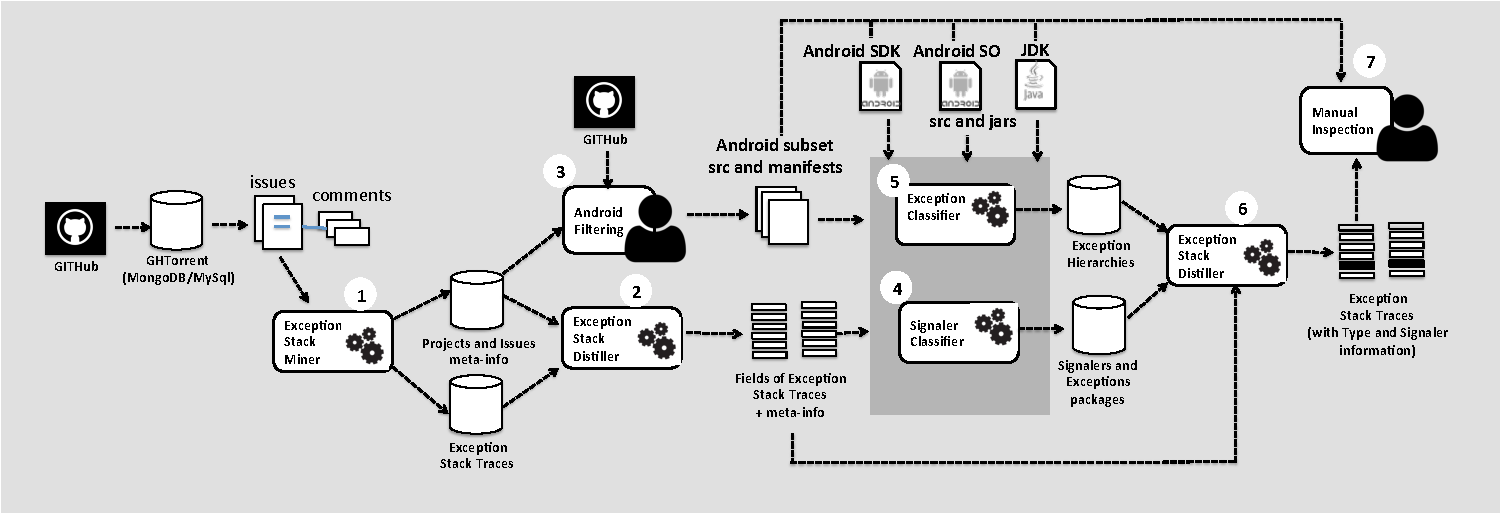
\includegraphics[width=\hsize]{overview.pdf}
\caption{Overview of the study based on mixed approaches.}
\label{fig:overviewfig}
\end{figure*}

%The GHTorrent dataset covers a broad range of
% development activities on Github, including the all the issues per project. Such data 
%is stored in unprocessed format, in a MongoDB database, while metadata is extracted 
%and stored in a relational database. 



\textbf{Step1.} To obtain the Dataset to be analized, we queried GHTorrent as detailed in Section XXX. From GHTorrent we retrieved the metadata related to each Java project (e.g., 
repository's names and short descriptions), and the content of every issue and issue comment 
and stored in a relational database.

\textbf{Step 2.} Extracting Exception Information from Issues. In this step, we used the ExceptionMiner tool,
 developed in this work, to extract the exception names and exception stack traces of each
 issue and issue comment - analyzing the information of each project at a time. This initial 
set of analyzed Java projects included libraries, web-based, Android and stand-alone applications.  

\textbf{Step 3.} Restricting the Dataset to Android Projects. We select a subset of all Android 
projects available on the dataset to perform a deeper analysis (which combined mined
 information extrated from issues with source-code analysis and manual inspection 
of projects resources described on next steps). This decision was driven by the
fact that most open source Anedroid applications are known for dealing
with several sources of exceptions due to multi-threaded execution and
interaction with input/output resources; moreover they share a common
well-defined platform and a limited set of libraries.
To identify Android projects, we performed a case insensitive search for 
the term \textsf{android} in the repository's names and short descriptions.  The
heuristic filtered 2.542 repositories, from which 589 apps had at least one
issue containing a stack trace. Then we performed further cleanup, inspecting the site of every Android
reporting at least one stack trace, to make sure that they represented real
mobile apps. During this clean up 106 apps were removed because they were either
example projects (i.e., toy projects) or tools to support Android development
(e.g. \textsf{selendroid}, \textsf{roboeletric} --- tools to support the testing of Android apps).
The filtered set consisted of 482 apps, from which approximately 50\% are also
hosted in Google Market Place. 

To support a deeper investigation of the stack traces of Android apps, every
exception defined on a stack trace was then classified according to its type
(e.g. Error, Exception or RuntimeException) and to its signaler. To do so, the following 
steps were performed:

\textbf{Step 4.}  Bytecode-Code analysis of JVM and Android Exceptions. We developerd a bytecode analysis tool based on DesignWizard to discover all exceptions thrown by the last version of SDK version 7, and Android Platform and OS (level 19). Every exception was extracted and classified as Runtime, Checked or Error based on the analysis of the exception hierarchy. Our analysis found XXX runtime exceptions in JVM and XX checked, on Android xxx checked and YYY runtime.

\textbf{Step 5.}  Source-Code Analysis of Android Projects. 
For each one of the analyzed projects, we
downloaded the source code and using custom scripts, we extracted their package
hierarchy (recursive list of of Java packages) and their custom exception types.

\textbf{Step 6.}  Manual Inspection. XXXX of the exceptions reported on stack traces  could not be found on JMV, SO or inside the last version of the project. Based on the full name of the exception, a manual inspection was performed on the artifacts associated to the project and libraries used by the project. When even on those sources the exception was not foung [grep-code and similar sites] the exception, in order to discover the exception type. Only 3 exceptions remained undefined and were removed from this study.

OBS: THE PICTURE WILL BE UPDATED TO REFLECT THIS PROCESS DESCRIPTION.

\subsection{The ExceptionMiner Tool}
\label{sec:exceptionminer}

To extract exceptions from issues, we implemented ExceptionMiner, a modular
mining tool able to connect to various repositories (such as Google Code,
GHTorrent or even directly to Bugzilla), extract issues, mine stack traces from
them and classify them in predefined categories. The main components of
ExceptionMiner are as follows:

\noindent\emph{StackTraceMiner and Distiller} The first step in the process is
mining references to exceptions and stack traces embedded in issues, distilling
the information that composes a stack trace and storing the results in a
relational database. Some of the information extracted from the stack traces were:
 the exception being thrown, its signaler, the exception root cause, its corresponding signaler,
and packages related to each one of these fields.
The tool is based on a combination between a regular expression based parser 
with heuristics able to identify and filter exception names and stack traces inline with text. In
contrast to existing issue parsing solutions such as Infozilla, the parser
created in this work can extract all causes related to an exception on a stack,
and stack traces embedded in logs files.

%\begin{tiny}
%\begin{verbatim}

%03-01 W/dalvikvm(7924): threadid=1: thread exiting with uncaught exception (group=0x40adf210)
%03-01 15:55:01.609 (7924): FATAL EXCEPTION: main
%03-01  (7924): java.lang.RuntimeException: ...
%E/AndroidRuntime( 7924):  at android....performLaunchActivity(ActivityThread.java:1967)
%03-01 15:55:01.609 (7924):  at android....handleLaunchActivity(ActivityThread.java:1992)
%03-01 15:55:01.609:  at android.app.ActivityThread.access\$600(ActivityThread.java:127)
%E/AndroidRuntime( 7924):  at android....handleMessage(ActivityThread.java:1158)
%\end{verbatim}
%\end{tiny}

\noindent\emph{Exception Classifier} The next step in the ExceptionMiner process
is classifying exceptions as either checked exceptions, runtime exceptions or 
errors. The exception classifier is based on bytecode analysis (based on Design
Wizard~\cite{Brunet09}) that walks up the type hierarchy of a Java exception
until it reaches a base exception type.

\noindent\emph{Exception Signaler Classifier} After its initialization it
classifies each signaler according to its origin (i.e. Android Plaform,
Aplication, Library, Libcore, or Java) based on pattern matching between the
signaler name and the packages associated to each category.

%\section{Study Operation and Results}
Next section presents the results for each of the study phases, providing both a
quantitative and qualitative analysis of the outcomes.


\section{RQ1: What are the common characteristics of such stack traces?}

%To answer this question, we mined from every extracted stack trace the top level
%exception being signaled, its signaler (the first method signature frame after
%the exception), the root exception (the exception which initiated the stack
%trace, defined on the bottom of the stack), and the root signaler. The
%intermediate elements that compose a stack trace as shown in
%Figure~\ref{fig:wrapping} (i.e., the intermediate causes and its execution
%stacks) were not be considered in the analysis.
%~\todo{Move this to the previous section? IMO, It is better to keep all facts
%about how we did the research in one place
%RSC: I WAS ABOUT TO MOOVE BUT THERE WAS ALREADY A SIMILAR TEXT ON 
%THE EXCEPTION DISTEILLER}

Based on the assumption that regardless the issue type, every exception stack
trace contains relevant information concerning the exception structure of
projects analyzed we opted for not restricting the analysis only on defect
issues.\footnote{We conducted the same analysis on the defect issues and the top
exceptions are similar to the ones mentioned on defect issues. Due to space
limitation we limit to present the general analysis here. More detailed analysis
on the defect issues can be found at:
\url{www.dimap.ufrn.br/~roberta/icsme2014}}

\subsection{Characterizing the Most Common Exceptions}

After distilling the information available on the 28,800 stack traces were extracted from the 
issues and issues comments of 16,836 Java projects: 607 distinct root causes were found, 
and  2,026 distinct top level exceptions were found.

From this set the java.lang.NullPointerException  was the root cause most 
reported;  7578 stack traces had a java.lang.NullPointerException  as root cause,
 which corresponds of 26,31\%  of all analyzed stack traces.

If we perform a cross-project analysis, the java.lang.NullPointerException, we could observe that such 
exception was reported on 1,671 projects (which represents 44,47\% of all projects reporting at least one stack trace).

The high prevalence of NullPointerExceptions is aligned with the findings other works~\cite{kim2013predicting,fraser20131600,csallner2004jcrasher}. For instance, Sunghun et
al.~\cite{kim2013predicting} showed that in Eclipse bug report system 38\% the bugs related to exception handling were caused by NullPointerException; other works on robustness testing~\cite{maji2012empirical,csallner2004jcrasher} showed that most of the automatically detected bugs were due to NullPointerExceptions and implicitly-signaled of Java
environment (as the ones found in this study).

To better understand the root causes reported on stacks, we performed a categorization 
study on which the top 100 root causes reported on stack-issues were manually inspected.
The characterization process consisted of classifiying each exception in one of the
chategories listed on Table X, based on the inspection of source code, Javadoc, 
or additional documentation related to the exception.

\begin{table}
  \centering
  \begin{tabular}{|p{2cm}| p{5cm}|}
    \hline
    \bfseries{Category} & \bfseries{Description} \\
    \hline
      Programming logic &  Exceptions implicitly  thrown by the JVM when the 
evaluation of an expression violates the normal semantics of language (e.g., 
out-of-bounds array index, division-by-zero, access to a null reference). 
Such exceptions are usually defined on java.lang and java.util packages. \\ \hline
      Resources (IO)                         & Exception releated to the manipulation of IO resources or device  (e.g., file, network) \\ \hline
      Security                               & Exception releated to security issues (e.g. password validation, criptography) \\ \hline
      Concurrency                            & Exceptions related to multi-threaded programming \\ \hline
      Backward compatibility                 &  A list of exceptions related to backward compatibility - a complete list can be found here [ref]  \\ \hline
      Reflection                             & Exceptions related to Java reflection library  \\ \hline
      Specific                & Exceptions created for specific applications, frameworks or libraries \\ \hline
      General (Exception, Error, Runtime)    & The top level exceptions in Java    \\ \hline
    \hline
  \end{tabular}
  \caption{Categories description.}
  \label{tab:categories}
\end{table}

The top 100 root causes correspond to approximately 77\% of all stack traces
reported reported on Java stack-issues and 95\% of all exceptions reported on
Android stack-issues. Table~\ref{tab:tophundrend} illustrates the result of such 
classification.

\begin{table}
  \centering
  \begin{tabular}{lrr}
    \hline
    \bfseries{Category} & \bfseries{Java} & \bfseries{Android Subset} \\
    \hline
      Programming logic (java.lang and util) & 12625  (41,10\%) & 2235 (55,64\%)\\
      Resources (IO)                         & 12440 (40,50\%)  & 727 (18,10\%) \\
      Security                               & 220  (0,72\%)    & 165 (4,11\%)\\
      Concurrency                            & 633 (2,06\%)     & 116  (2,89\%)\\
      Backward compatibility                 & 1580 (5,14\%)    & 219 (5,45\%) \\
      Reflection                             & 1413 (4,60\%)    & 91 (2,27\%)\\
      Specific (GUI,FRAMEWORK)               & 340 (1,11\%)     & 197 (4,90\%)\\
      General (Error, Exception, Runtime)    & 1468 (4,78\%)    & 267 (6,65\%)\\
    \hline
  \end{tabular}
  \caption{Characterization of the 100 root causes.}
  \label{tab:tophundrend}
\end{table}

Programming errors are the causes of most of the exception stack traces reported
on issues. In the Android subset we could find more issues related to Backward
compatibility and security issues than on the general data set.


\subsection{Investigating Android Subset}

As detailed in Section~\ref{sec:android}, 482 Android projects were carefully
selected to enable a deeper investigation of stack trace information, by
leveraging stack trace information with the source code and bytecode analysis.
For this subset of Android project, we could extract every package related to
each exception signaler, and based on this information we could classify every
stack trace based on its root signaler as presented in Table~\ref{tab:signalers}.

\begin{table}
  \centering
  \begin{tabular}{rp{29em}}
    \hline
    \bfseries{Signaler} & \bfseries{Description} \\
    \hline
    \bfseries{android} & If the exception is thrown by a method defined in Android Platform or OS, or in a JDK library used by them.\\
    \bfseries{app}     & If the exception is thrown by an application method or in a  DK library used by it.\\
    \bfseries{libcore} & If the exception is thrown by one of the core libraries reused by Android (i.e., org.apache.harmony, org.w3c.dom, sun.misc, org.apache.http, org.json, org.xml). \\
    \bfseries{lib}     & If the exception is thrown by a method that was not defined by any of the elements above.\\
    \bfseries{java}    & If all methods on the stack trace are JDK library methods.\\
    \hline
  \end{tabular}
  \caption{Sources of exceptions in Android}
  \label{tab:signalers}
\end{table}

For each exception we could discover the number of times it occurred on stacks,
the number of distinct projects on which such stacks were defined (and consequently its
popularity) and the of times it was signaled by different signaler types. We
could calculate the popularity of each root cause, considering the number of
distinct projects they were found and the whole set of projects analyzed with at
least one stack trace (482). Table~\ref{tab:toptenandroid} 
%and Figure~\ref{fig:androidsignaler}
presents the mined data.

\begin{table*}
  \centering
  \begin{tabular}{rccccccccc}
    \hline
    \bfseries{Root Exception} &  \multicolumn{2}{c}{\bfseries{Occurrences}} &  \multicolumn{2}{c}{\bfseries{Projects}} & \textsf{android} & \textsf{libcore} & \textsf{app} & \textsf{lib} & \textsf{java} \\
    & \bfseries{\#} &  \bfseries{\%} & \bfseries{\# } & \bfseries{\% } &&&&&\\
    \hline
java.lang.NullPointerException            & 1225 & 30,08\% & 254 & 52,70\% & 473 & 18 & 595 & 137 & 2 \\
java.lang.IllegalStateException           & 234  & 5,75\%  & 99  & 20,54\% & 165 & 12 & 36  & 20  & 1 \\
java.lang.IllegalArgumentException        & 255  & 6,26\%  & 94  & 19,50\% & 146 & 6  & 64  & 39  & 0 \\
java.lang.RuntimeException                & 232  & 5,70\%  & 91  & 18,88\% & 167 & 1  & 47  & 17  & 0 \\
java.lang.OutOfMemoryError                & 180  & 4,42\%  & 56  & 11,62\% & 121 & 15 & 17  & 23  & 4 \\
java.lang.NoClassDefFoundError            & 73   & 1,79\%  & 52  & 10,79\% & 9   & 0  & 37  & 26  & 1 \\
java.lang.ClassCastException              & 94   & 2,31\%  & 49  & 10,17\% & 43  & 0  & 40  & 11  & 0 \\
java.lang.IndexOutOfBoundsException       & 127  & 3,12\%  & 47  & 9,75\%  & 47  & 0  & 71  & 8   & 1 \\
java.lang.NoSuchMethodError               & 57   & 1,40\%  & 40  & 8,30\%  & 9   & 0  & 39  & 9   & 0 \\
java.util.ConcurrentModificationException & 54   & 1,33\%  & 38  & 7,88\%  & 5   & 0  & 43  & 6   & 0 \\

    \hline
  \end{tabular}
\caption{Root Exceptions occurrences and popularity.}
\label{tab:toptenandroid}
\end{table*}

%\begin{figure}
%\centering
%\includegraphics[width=\hsize]{top_exceptios_android_new2.pdf}
%\includegraphics[width=\hsize]{top_exceptions_android_new}
%\caption{Top exceptions in Android repositories.}
%\label{fig:androidsignaler}
%\end{figure}

Programming mistakes are the most common root causes for most types of signalers. We
could observe that the NullPointerException is still the exception with higher
number of occurrences. The NullPoiterExceptions are mainly signaled inside
Android platform and inside application code, although we also find
NullPointerExceptions being signaled from third-party libraries. Regarding
reusable code, there is no consensus whether it is a good or bad practice to 
re-throw
a NullPointerException. Some prefer to encapsulate such an exception on
IllegalArgumentException, while others~\cite{bloch2008effective} argue that the
NullPointerException makes the cause of the problem explicit and hence 
should not be wrapped.

We could observe in this study that the NullPointerException and other
other implicitly signaled exceptions represented most of the exceptions reported
on issues in both Java and Android subset. For such exceptions, which represent
programming bugs or resource limitations, there is usually no proper handling
besides presenting an error message to the user and restarting the application.
Only high fault tolerant systems need to provide solutions to handle them.



%\subsection{Sizes of Stack traces}
%Concerning the size of the stacks (i.e. the number of frames composing them), we
%could observe that  sometimes it exceeded 100 frames (158 stack frames).
%Manually inspecting the corresponding execution trace was caused by one of the
%two reasons: recursive calls or exceptions signaled by a method defined deep
%down in a reused framework; exceptions successively wrapped. Irrespective of the
%reason, in exception flows involving many methods, it is practically impossible
%to handle an exception in a way other than exiting the application, as at the
%place the exception occurs there is hardly enough contextual information to
%perform recovery actions.

%Considering only the packages of each exception we could observe that 81,28\%
%of all analyzed set of stack traces reported exceptions defined by java.lang
%(see Table XXX).

%\begin{table}
% \centering
%\begin{tabular}{lrrrr}
%    \hline
% \bfseries{rank} & \bfseries{package} & \bfseries{occurr} &  \bfseries{\%occur} & % \bfseries{projects} \\
%     \hline
%1 & java.lang         & 19471 & 81,28\% & 3080 \\
%2 & java.io           & 1222  & 5,10\%  & 509 \\
%3 & java.net          & 740   & 3,09\%  & 311 \\
%4 & java.util         & 689   & 2,88\%  & 287 \\
%5 & java.lang.reflect & 115   & 0,48\%  & 78 \\
%\hline
%  \end{tabular}
%\caption{Top 5 most popular packages associated to the root exceptions of stack traces}
%\label{tab:toptenpopular2}
%\end{table}

%\noindent \fbox{
%\begin{minipage}{0.96\columnwidth} 
%\emph{RQ2: Most exceptions are due to programming mistakes
%or generally irrecoverable errors.}
%\end{minipage}}

\section{RQ2.  What kinds of exception (mis)-use emerge from stack trace analysis? }

To answer this question we analyzed general characteristics of reported stack traces and, in the case of stack traces reported on Android repositories, we combine stack trace information with
source code and byte code analyses to enable a more detailed analysis.
Doing so, we mined some characteristics of stacks that points to best practices violations.

\subsection{Direct instances of RuntimeExceptions being thrown.}

From Tables~\ref{tab:toptenjava} and~\ref{tab:toptenandroid} we can observe that,
in both Java and Android related issues, direct instances
java.lang.RuntimeException were thrown  in 10,94\% of Java repositories and
18,88\% of Android repositories respectively. 
In the Android repositories, most of such exceptions  were  thrown by the Android 
platform/OS (167 out of 232).

Throwing general exceptions, such as direct instances of RuntimeException, is  considered a
bad practice, because the exception type does not carry enough information to identify the
cause of the exceptional behaviour, and as a consequence developers need to relying on
the exception message which can be neither complete nor precise~\cite{gosling2000java}.


\subsection{Undocumented runtime exceptions being thrown.}

To better investigate the extent of this problem we classified each stack trace according to the type of the
root exception. Table~\ref{tab:typeroottab} presents the types of root causes of all stack traces reported on 
the Android repositories. As we can see from Table ~\ref{tab:typeroottab},  most of the exceptions signaled by third-party code
 (e.g., Android and libs) were runtime exceptions. After filtering all the exceptions implicitly signaled by 
JVM (due to programming mistakes) and inspecting the signaler methods of such exceptions (i.e.,  direct an indirect 
instances of java.lang.RuntimeException). We could observe that only 1 method out of 118 inspected signalers
 (i.e., 0,8\%) documented the explicitly thrown runtime exception in a Javadoc comment; and none of these methods
included the runtime exception  (reported on the stack) as part of the exception interface of the method (i.e., using 
throws clause on method signature). This result is aligned with the results of other  study conducted by from 
Sacramento et al ~\cite{sacramento2006unchecked} which observed that the
runtime exceptions in .Net programs are most often not documented.

Such undocumented runtime exceptions represent a threat to system robustness, specially
when such exceptions are thrown then the third party code is invoked inside the application (e.g. libraries, or framework utility code).
In such cases the client usually do not have access to the source code, and in the absence of
the exception documentation it is very difficult or even impossible for the client of such third party code to 
protect the application against undocumented runtime exceptions. As a consequence, the
 undocumented runtime exception may remain uncaught and lead to system crashes.

\begin{table}
\centering
\begin{tabular}{lcccccc}
    \hline
    \bfseries{Type} & \bfseries{Android} & \bfseries{Libcore} & \bfseries{App} & \bfseries{Lib} & \bfseries{Java} & \bfseries{All}\\
    \hline

Runtime	&	1075	&	56	&	1446	&	374	&	10	&	2961	\\
Error	&	144	&	34	&	168	&	105	&	9	&	460	\\
Checked	&	110	&	230	&	139	&	145	&	12	&	636	\\
Throwable	&	0	&	0	&	1	&	0	&	0	&	1	\\
Undefined	&	1	&	0	&	6	&	8	&	0	&	15	\\
    \hline
All		& 1330	&	320	&	1760	&	632	&	31	&	4073	\\
    \hline
  \end{tabular}
\caption{Types of root exceptions.}
  \label{tab:typeroottab}
\end{table}


\begin{figure}
\centering
%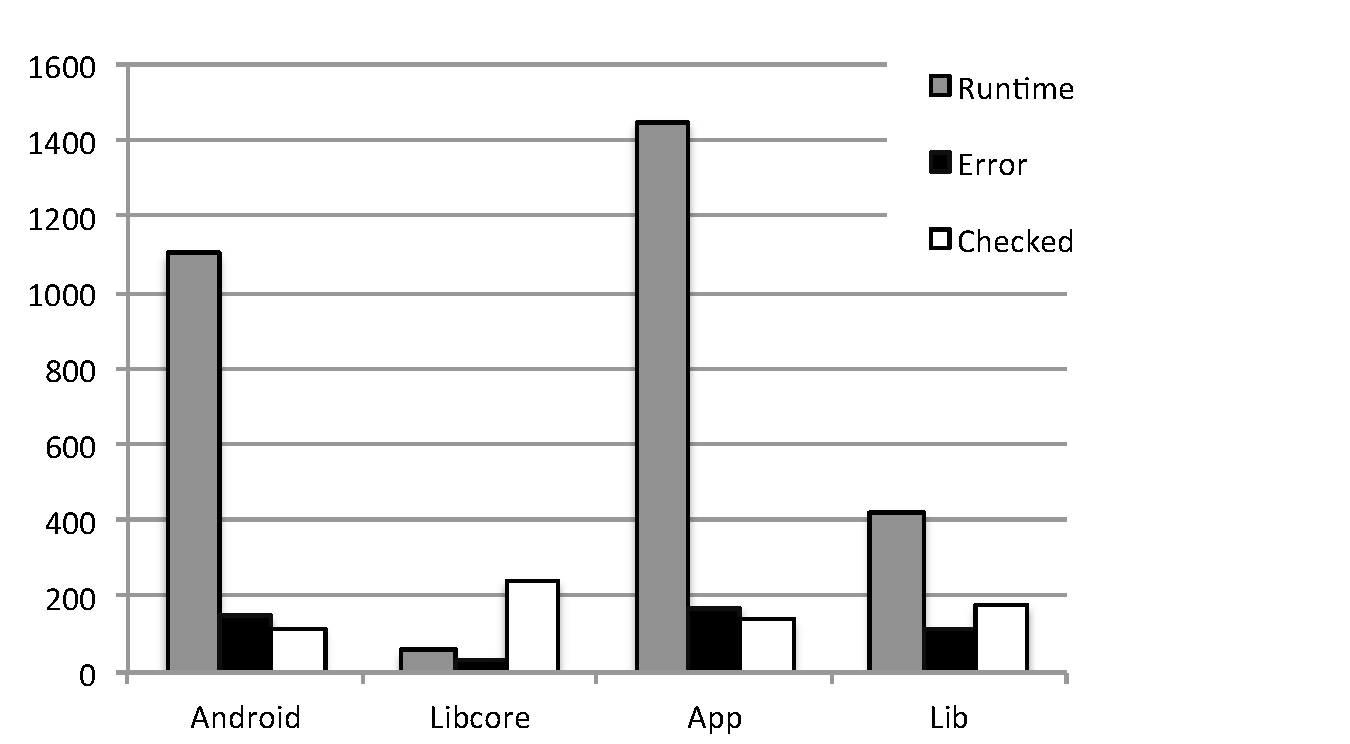
\includegraphics[width=\hsize]{chart_exceptiontypes.pdf}
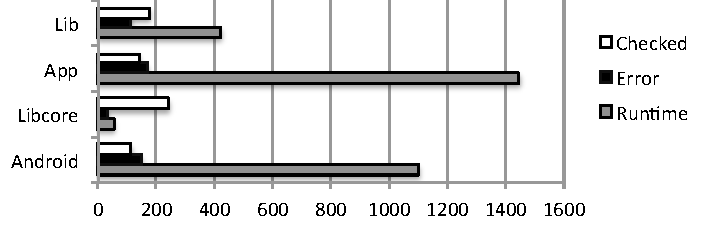
\includegraphics[width=\hsize]{exception_types.pdf}
\caption{Distribution of Checked and Unchedked exceptions.}
\label{fig:typeroot}
\end{figure}

On the other hand, we could observe that most of the exceptions signaled by the set of 
libraries reused by Android platform (i.e., org.apache.harmony,
org.w3c.dom, sun.misc, org.apache.http, org.json, org.xml, javax -- referred in
this work as libcore) were checked exceptions. It is pointed as a good practice
for libraries (see Section~\ref{sec:best}) because by using checked exceptions
libraries can define a precise exception interface to its clients. Such
libraries are heavily used in several projects, and such precise exception
interface may be related to the library's maturity.

\subsection{Uncaught Checked Exceptions}

Although most of the  reported exceptions were runtime, we could also find checked
exceptions as the root causes of stack traces reported on issues. A checked exception
can remain uncaught in two circumstances: if all methods on the execution trace
on which this exception flows explicitly specifies the exception, or if the
checked exception is wrapped in a runtime and than re-thrown. Since checked exceptions 
should be used to represent recoverable conditions, ignoring a
checked exception, is considered a bad practice. As mentioned before, when the developer is confronted
with a checked exception, the designer of the API is telling him to handle the
exceptional condition. To better understand what was causing checked exceptions
to scape from being handled we investigated the kinds of wrappings that happened
on stacks the stacks.  Next sections presents the wrappings found and discuss
about them.

%\noindent\emph{3) Odd Wrappings}
\subsection{Odd Wrappings}
Table~\ref{tab:wrappingandroid} presents the wrappings found in this study for all
stack traces found in Android repositories. As we can see, some of the checked
exceptions where indeed wrapped in runtime exceptions or even errors, while most
of them were not wrapped along the stack trace. 

\begin{table}
\centering
\begin{tabular}{llll}
    \hline
    \bfseries{Root Cause} & \bfseries{Wrapper Type} & \bfseries{Occurrences} & \bfseries{Projects} \\
    \hline
     Runtime    & -   &  2360 & 359 \\

    Runtime   & Runtime & 560  & 182 \\
    
 Checked    &   -  & 422  & 117 \\
     Error    &   -   & 381  & 141 \\
   Checked &  Runtime   & 109  & 70  \\
    Checked   & Checked & 98   & 42  \\
   Error   &  Runtime   & 55   & 38  \\
   Runtime &  Checked   & 22   & 12  \\
    Error     & Error   & 15   & 14  \\
  Undefined    &  -  &  15   & 10  \\
   Runtime & Error     &  13   & 6 \\
  Error   & Checked   &  8    & 7 \\
    Checked &Error     &  7    & 4 \\
    Runtime &Throwable &  3    & 1 \\
   Runtime & Undefined &  3    & 3 \\
   Throwable    & -  &  1    & 1 \\
   Error   & Undefined &  1    & 1 \\
    \hline
  \end{tabular}
\caption{Kinds of wrappings found on the stacks of 482 ANDROID projects found on Github}
\label{tab:wrappingandroid}
\end{table}

This analysis also revealed unexpected wrappings such as: Error wrapping a Checked 
exception; a Runtime wrapping and Error; and an Error wrapping a Runtime.
Java is the only language that provides a hybrid exception handling mechanism
which offers  different types to represent different exception behaviors (i.e., error, 
runtime and checked) (see Section~\ref{sec:best}). According to Java specification Errors should not be
handled inside the system since they usually represent unrecoverable conditions
detected by the JVM such as OutOfMemoryError. Checked exceptions should
represent recoverable conditions and  Runtime exceptions represent are usually
related to programming mistakes from which the developer is not expected to recover
from. 

%Table X illustrated examples of such wrappings.
%TODO INCLUIR ESTA TABLEA

%\begin{figure}
%  \begin{center}
%    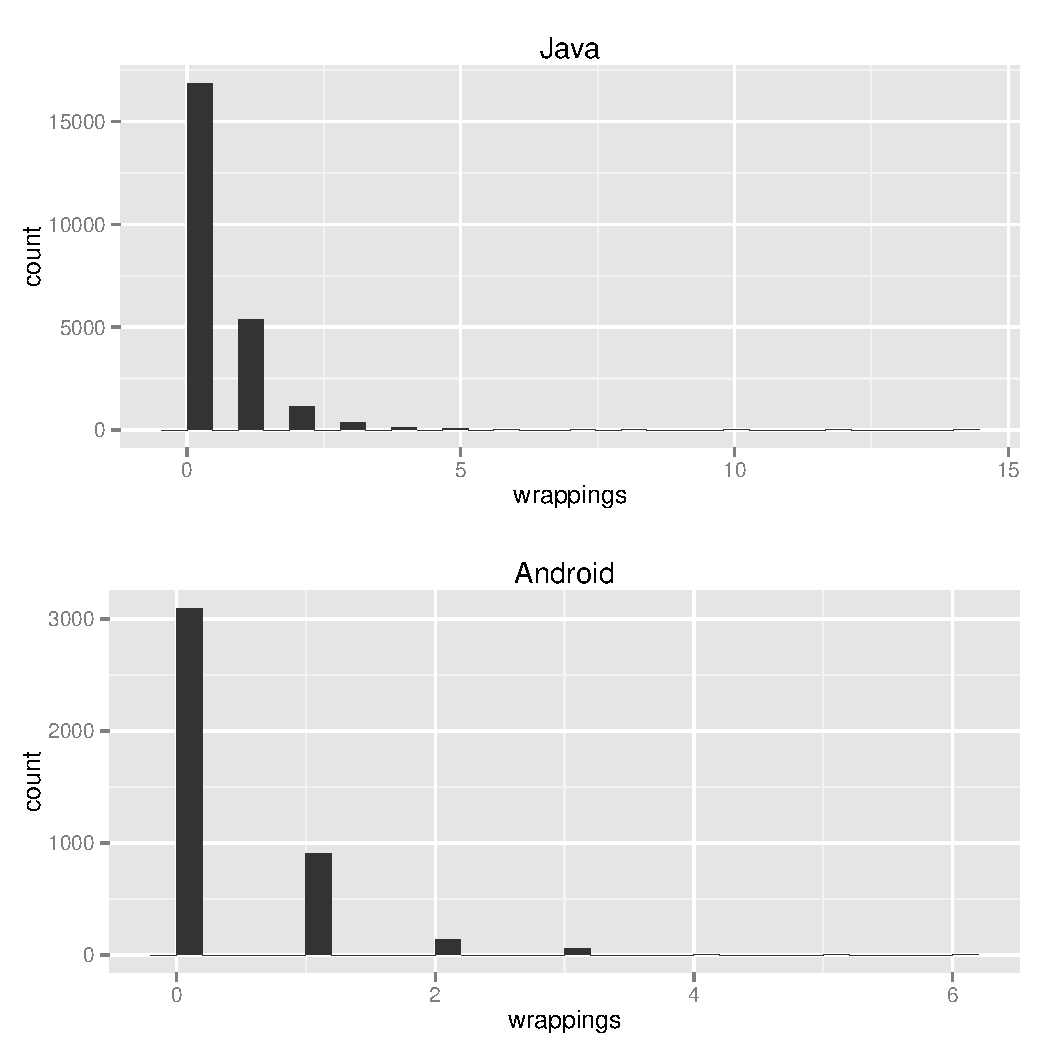
\includegraphics[scale=0.4]{stack-wrappings-hist.pdf}
%  \end{center}
%  \caption{Number of stack traces wrappings for Java and Android repositories. }
%  \label{fig:sizewrapbhists}
%\end{figure}

We could also observe that in 205 stacks found in Android repository the exception was wrapped 
more then once. Figure ~\ref{fig:sizewrapbhists}  illustrates the number of wrappings per stack, both
 in Java and Android studied repositories. One interesting multiple-wrapping found in Android repo was the 
following: Runtime-Checked-Runtime-Checked-Runtime-Checked-Runtime.

Since there is no way of enforcing Java exception type conventions during program development,
we could observe the stack trace analysis combined with types these three types
of exceptions were used interchangeably. This interchangeability makes the
behaviour of the exception handling code more complex and less reliable. For
instance, considering a situation were an instance of OutOfMemoryError (a situation that
should not be handled) was wrapped in a checked exception (a situation that must
he handled), in this case this wrapping is telling to the caller that it should
handled.

\section{Discussion}

The exception (mis-)use patterns that emerged  in this study sheds light on 
problems that may be reducing the robustness of current Java programs in the face of
exceptional conditions. \noindent\emph{The undocumented runtime exceptions} thrown by library code -
documenting runtime exceptions is a tedious and error prone task, to help developers
mitigate this problem tools should be developed to automate the documentation of runtime exceptions
scraping from library code, few solutions in this directions have been proposed so far ~\cite{van2005combining}. 
 \noindent\emph{The odd wrappings}  found in this study can lead to what we call
an \emph{exception handling confusion problem} which can lead the program to
an unpredictable state in the presence of exceptions. To illustrate this problem, we can use
 one of the examples found in this study: when the developer is 
confronted with a checked exception, the designer of the API is telling him 
to handle the exceptional condition, however we could observe that in some cases the 
checked exception wrapped an OutOfMemoryError, which represent resource deficiency detected 
by the JVM which make impossible the program to recover. Further investigation is needed on finding 
ways to help developers in deadling with such problem, either preventing odd wrappings or enabling 
the developer to better dealing with them. Last but not least, the high number of null pointer exceptions 
lead us to think on other pertinent research direction: whether language designs which avoid null pointers, 
such as Monads ~\cite{Walde95} (i.e., used in functional languages for values that may not be available 
or computations that may fail) could improve the robustness of Java programs. 



TO DISCUSS: How can we benefit from such cross-project crash analysis?



\section{Threats to Validity}

\noindent\emph{Internal Validity} We used a heuristics-based parser to mine
exceptions from issues.  Our parsing strategy was conservative by default; for
example, we only considered exception names using a fully qualified class name
as valid exception identifiers, while, in many cases, developers use the
exception name in issue description. Conservative parsing may minimize false
positives, which was our initial target, but also tends to increase false
negatives, which means that some cases may have not been identified as
exceptions or stack traces. Our limited manual inspection did not reveal such
cases.

\noindent\emph{External Validity} The results presented here were based on mining
issues on Github through the GHTorrent dataset. While comprehensive and
extensive, GHTorrent is not an exact replica of Github, so several issues might
be left out. Due to the way data collection works with GHTorrent, for projects
that are relatively inactive, GHTorrent might have not collected a significant
proportion of their issues. We did not investigate the extend of this threat on
our sample.

\noindent\emph{Construct Validity} Parts of our analysis are based on the availability of stack traces on issues on
Github. In using this dataset, we make an underlying assumption: the
stack traces reported on issues are representative of real crashes in
the applications. The assumption is impossible to mitigate without access to
the full set of crash data per application. Services exist to collect all
crash data from applications, so access to such a dataset will allow for
a thorough replication of our analysis, perhaps at the individual application
level.

\section{Related Work}

In this section, we present work that is related to the present paper, divided into
three categories: i) papers that use the information available on stack traces;
ii) empirical studies on the usage of Java exceptions and its fault proneness;
and iii) tools to extract stack traces information from natural language artifacts
(e.g., issues and emails).
%, and iv) empirical studies involving Android apps.

\textit{Analysis of Java Exception Usage.} As the manual analysis of the Java
exception flow can easily become infeasible, Robillard and Murphy~\cite{Robil00}
employed dataflow analysis to find the propagation paths of checked and
unchecked exception types. Modeled after Robillard and Murphy's work, other
tools have been proposed to support the static analysis of exception
flows~\cite{coelho2008assessing}. The main limitation of all
static analysis tools is the number of false positives inherent to static analysis
solutions, which can lead to a high number of exception flows, specially if
considering Java Environment exceptions and exceptions signaled from libraries.
Additionally, Cabral and Marques~\cite{cabral2007exception} analyzed the
exception handling code of 32 open-source systems, both for Java and .NET. They
observed that the action handlers were very simple (e.g., logging and present a
message to the user). Reimer and Srinivasan~\cite{reimer2003analyzing} listed a
set of bad practices on exception handling that hinder software maintainability
and robustness, based on their own experience with Java enterprise applications.
Our work differs from those two works as we tried to identify bad practices from
the combined use of stack traces extracted from issues and bytecode and source
code analysis. 

\textit{Analysis and Use of Stack Trace Information.} Several works have
investigated the use of stack trace information to support bug classification
and clustering~\cite{wang2013improving, kim2011crash, dhaliwal2011classifying},
fault-proneness prediction models~\cite{kim2013predicting} and even automated
bug fixing tools~\cite{sinha2009fault}. Kim et al.~\cite{kim2011crash} use an
aggregated form of multiple stack traces available in crash reports to detect
duplicate crash reports and to predict if a given crash will be fixed. Dhaliwal
et al.~\cite{dhaliwal2011classifying} proposed a crash grouping approach that
can reduce bug fixing time in approximately 5\%. Wang et
al.~\cite{wang2013improving} propose an approach to identify correlated crash
types and describe a fault localization method to locate and rank files related
to the bug described on a stack trace. Schroter et al.~\cite{schroter2010stack}
conducted an empirical study on the usefulness of stack traces for bug fixing
and showed that developers fixed the bugs faster when failing stack traces were
included on bug issues.  In a similar study, Bettenburg et
al.~\cite{bettenburg2008makes} identify stack traces as the second most stack
trace feature for developers.  Sinha et al.~\cite{sinha2009fault} proposed an
approach that uses stack traces to guide a dataflow analysis for locating and
repairing faults that are caused by the JVM implicitly signaled exceptions. Kim
at al.~\cite{kim2013predicting} proposed an approach to predict the
crash-proneness of methods based information extracted from stack traces and
methods' bytecode operations.  They observed that most of the stack traces were
related to NullPointerException and other JMV implicitly thrown exceptions had
the higher prevalence on the analyzed set of stacks.

\textit{Extracting Stack Traces from natural language artifacts.} 
%Currently, many
%software vendors embed automatic crash reporting tools in their software
%systems. Moreover, third party crash collection services exist, most of them 
%targeted for applications run on mobile phones~\cite{BugSe14,BugSn14,Googl14,Acra14}.
Apart from bug reports, stack traces can be embedded in other forms of
communication between developers, such as discussion logs and emails.
Being intermixed with text makes the accurate extraction of stacktraces 
an involved process.
Infozilla~\cite{bettenburg2008extracting}
is based on a set of regular expressions that extract a set of frames
related to a stack trace. The main limitation of this solution is that it is not
able to extract stack traces embedded on verbose log files (i.e., on which we
can find log text mixed with exception frames). Bacchelli
et al.~\cite{bacchelli2012content} propose a solution to recognize stack trace frames
from development emails and relate it to code artifacts (i.e. classes) mentioned
on the stack trace. In addition to those tools, ExceptionMiner is able to 
both extract stack traces from natural language artifacts and to 
classify them in a set of predefined categories.

%\textit{Empirical studies using Android apps.} Ruiz et al.~\cite{Ruiz12}
%investigated the degree of reuse across applications in Android Market, the
%study showed that almost 23\% of the classes inherited from a base class in the
%Android API, and that 217 mobile apps were reused completely by another mobile
%app. Pathak et al.~\cite{Patha11} analyzed bug reports and developers
%discussions of Android platform and found out that approximately 20\% of
%energy-related bugs in Android occurred after an OS update. McDonnell et
%al.~\cite{McDon13} conducted a case study of the co-evolution behavior of
%Android API and 10 dependent applications using the version history data found
%in github. The study found that approximately 25\% of all methods in the client
%code used the Android API, and that the methods reusing fast-evolving APIs were
%more defect prone then others. Vásquez et al.~\cite{Linar13} analyzed
%approximately 7K free Android apps and observed that the last successful apps
%used Android APIs that were on average 300\% more change-prone than the APIs
%used by the most successful apps. Pingyu and Elbaum~\cite{Zhang12} analyzed bug
%reports of 5 Android applications an observed that 29\% had to do with poor
%exceptional handling code. Our work differs from the others as it aims at
%distilling the information of bug reports describing uncaught exceptions created
%for mobile applications in Github, in order to get a first view
%of what is causing the crashes across applications available and what the
%characteristics of the stack traces can tell us about the exception structure of
%those applications.

\enlargethispage{-2\baselineskip}

\section{Conclusion}

In this paper we present an exploratory study in which we mined the stack 
traces embedded in all issues of Java projects available GitHub.
Furthermore, we analyzed in more detail the
stack traces reported on a subset of 482 Android projects. In this study, the information extracted 
from stack traces was used in combination with source code and bytecode analysis to 
pin-point patterns of exception use and misuse in Java.
Certain patterns of exception
(mis)-use were consistently detected such as unexpected wrappings (e.g., Errors
being wrapped in checked exceptions), revealing that  the Java hybrid exception
model is not fully used according to its purpose; undocumented runtime
exceptions signaled by third party code (which makes it almost impossible for
library clients to protect against such exceptions); 
and a high prevalence of
\texttt{java.lang} exceptions reported on issues (representing approximately 50\% of the
analyzed issues). Such (mis)uses detected in our study can negatively affect the 
robustness of current Java software systems. Our results call for  
 developing tools support to help developers dealing with such problems and 
improving the design of the exception handling mechanism in Java.

%Nowadays many software vendors embed automatic crash reporting tools in their
%software systems. Hence, whenever a software crashes this tool sends a detailed
%crash report to its vendors. Moreover, we can also find third party sofware
%solutions specialized in bug reporting for different kinds of systems specially
%for the increasing marked of mobile apps~\cite{BugSe14,BugSn14,Googl14,Acra14}.
%There is planty of information to be mined...


\section*{Acknowledgment} This work is partially supported by: CNPq -- Proc.
484209/2013-2 and the NWO TestRoots project (639.022.314).


\section {Old Introduction}



....... OLD VERSION ......

Modern applications have to cope with an increasing number of abnormal
computation states that arise as a consequence of faults in the application
itself (e.g., access of null references), noisy user inputs or faults in
underlying middleware or hardware. The exception handling
mechanism~\cite{goodenough1975exception} is one of the most used schemes for
detecting and recovering from such exceptional conditions. Although the
exception handling mechanism has been embedded in several programming languages
(e.g. Java, C++, C\#) and was the target of several studies
(e.g.~\cite{miller1997issues,Robil00,shah2010understanding,
garcia2007extracting,garcia2001comparative,cabral2007exception,coelho2011unveiling}),
the exception handling code is often generally poorly understood and the least
tested part of software systems.

Often exception handling constructions may lead the developers into believing that
by just re-throwing and possibly logging the exceptions they can forget about the exceptional
situations during the development of the "happy path". This "ignore-for-now"
approach may turn the exception handling into a generalized "goto"
mechanism~\cite{mandrioli1992advances} making the program more complex and even
less reliable. This behaviour may lead to the problem of uncaught exceptions~\cite{jo2004uncaught}, one of the main causes of application crashes.

Moreover, some languages use exceptions to represent programming mistakes
(array index out-of-bounds, division-by-zero, dereferencing null pointers). In these cases,
exceptions are implicitly signaled by the runtime environment when such
conditions occur. One of such implicit exceptions (caused by data conversion
from a 64-bit floating point to a 16-bit signed integer) was responsible for
the infamous failure on Ariane 5's first test flight~\cite{lions1996ariane} ---
leading to the rocket self-destructing 37 seconds after launch and a loss of 500
million dollars. Besides Ariane 5, several applications crash everyday due to
uncaught exceptions~\cite{jo2004uncaught}. Not using exceptions carefully
may have the opposite effect of the initial intention of improving
system robustness.

In Java, when the program fails due to an uncaught exception, it automatically
terminates, while the system prints a stack trace to the console. A stack trace
includes an explanatory message and the execution stack frame when the exception
occurred. A typical Java stack trace consists of an ordered list of methods that
were active on the call stack before the exception occurred. Stack traces
are a useful source of information about system crashes, and are often used to
support developers in debugging~\cite{schroter2010stack}. Moreover, information
from stack traces combined with crash and bug reports can be used to support bug
classification and clustering~\cite{wang2013improving, kim2011crash,
dhaliwal2011classifying}, fault-proneness prediction
models~\cite{kim2013predicting} and even automated bug
fixing~\cite{sinha2009fault} tools.

However, all existing research has focused on the analysis of a single system at a time. In
our current context, on which we have access to wealth of information available
on open-source repositories like GitHub additional questions arise: What is the
prevalence of exception stack traces on reported issues? What are the common
characteristics of such stack traces?

%What the stack traces available in these repositories can tell us about the use
%of exceptions in Java programs?

%To guide the our study we also compile general guidelines on how to use
%exceptions proposed by Gosling~\cite{gosling2000java},
%Wirfs-Brock~\cite{wirfs2006toward} and Bloch~\cite{bloch2008effective} and then
%we investigate: what stack traces can tell us about the adherence to such
%practices in Java programs?

To answer these questions, we conduct an exploratory study of stack traces in
the wild. Using a custom tool called ExceptionMiner, which was specifically
developed for this study, we mined stack traces from issues across all Java
projects on GitHub. Overall, we analyzed 356,057 issues from 16,836 projects,
from which 28,800 stack traces were extracted and used as a source of
information for our analysis. The stack trace analysis  was augmented by
additional information extracted using byte code and source code analysis done
on a carefully selected subset of our initial sample (482 Android projects).
%This study was divided in two phases: in the fist phase all the issues of all
%Java projects available on GitHub were analyzed and the embedded stack traces
%extracted using ExceptionMiner.

To guide this exploration we compiled general guidelines on how to use
exceptions proposed by Gosling~\cite{gosling2000java},
Wirfs-Brock~\cite{wirfs2006toward} and Bloch~\cite{bloch2008effective} and then
we investigate what stack traces can tell us about the adherence to such
practices in Java programs.
%~\todo{This should be our motivation, as this is
%our biggest contribution. I already changed the text. Lets discuss about this
%new version}
%RSC: I AGREE.


%GGG: I think this is too much detail for the introduction In the second phase
%of this study, we combined the information of the mined stack traces with
%source code and bytecode analysis. To do so we selected the subset of 482
%Android repositories. The Android repositories were chosen because this kind of
%application is known for dealing with several sources of exceptions, as they
%are usually io-intensive (i.e., deals with Network, Bluetooth, camera, and
%other resources), and multi-htreaded. Moreover, they are based on a single
%platform which allowed more fine-grained analysis of their exception behaviour.
%RSC: I AGREE.



This study builds upon the following assumption: the stack traces reported on
issues contain relevant information related to system crashes. Several studies
and techniques have also taken this assumption as starting point
(e.g.,~\cite{sinha2009fault}~\cite{dhaliwal2011classifying}~\cite{kim2013predicting}). Some outcomes were consistently detected through
our large scale analysis of exception stack traces in the wild, such as:

\begin{itemize}

  \item  A multitude of programming mistakes which are the main causes of stack traces.
   
  \item Undocumented runtime exceptions signaled by third party
    code (i.e., libraries and Android platform).

  \item  Odd exception chains (e.g., Error wrapping checked and runtime
    exceptions and vice-versa), indicating that the purpose of Java's hybrid
    exception model may not have been adequately used.

  \item  Stack traces caused by uncaught checked exceptions.

\end{itemize}

Hence, the contributions of this study are as follows:
\begin{itemize}

  \item  It performs the first large scale analysis of Java stack traces and how
    they can reveal bad-practices on the use of exceptions in Java.

  \item  It introduces ExceptionMiner, a tool developed to support cross-repository stack trace
    analysis.

\end{itemize}

These contributions are relevant to:
(i) developers of Java applications
to familiarize with the most common reported exceptions mis-uses which is the
first step to help developers to avoid making them; 
(ii) designers of languages
to consider ways of reducing the abundance of NullPointerExceptions;
and (iii)
tool designers to consider developing tools that enable a cross-project defect
analysis. 

% AVD: We have not looked at private issues, and the tool is described above.
%We strongly believe that, specially in the open-source environment,
%faults are not to be hidden in a private bug issue. Faults should be shared and
%discussed, so that a developer can learn from other projects mistakes.
%Currently, the search facilities of repositories are very limited, and the
%ExceptionMiner tool is a contribution in this direction.

%GGG: Personally, I hate this paragraph in all papers as it usually reads like a space-filler
%RSC: If needed we can remove it.
This paper is organized as follows. Section 2 presents a
background on exception handling mechanism. Section 3 presents the study design.
Section 4 reports study findings. Section 5 provides further discussions and insights.
Section 6 presents the threats to validity associated to this study. Finally Section
7 describes the related work, and Section 8 presents our conclusions and
directions for future work.




\subsection{Tentative  Introductions to chance the focus}

Along the recent years we have witnessed a rapid increase in 
the number of open source software  available on the Web.
Since such projects make their control version and 
issue tracking systems publicly available, they represent a valuable 
source of information for the "state of practice" on software development
which had already started to be investigated [][][][][][I still need to collect these references].

In this scenario Github emerged as one of the most used repository hosting sites.
It  alows developers to create and maintain opensource projects relying on Git distributed version 
control and provides a set of tools which allow the information about developers 
and their activities to be visible within and across open souce projects.

Bug issues have called the attention of the research community and have been the target of increasing 
researches [][][]. A specific type of bug issue is the one related to system 
crashes.  Such issues usually contain an exception stack trace [ref-paper], which tipically consists 
of an ordered list of methods that were active on the call stack before the failure occurred [ref-bug-issues]. 

Exception stack traces are a useful source of 
information about system crashes, and are often used to
support developers in debugging~\cite{schroter2010stack}. Moreover, information
from stack traces combined with crash and bug reports can be used to support bug
classification and clustering~\cite{wang2013improving, kim2011crash,
dhaliwal2011classifying}, fault-proneness prediction
models~\cite{kim2013predicting} and even automated bug
fixing~\cite{sinha2009fault} tools.

Although modern applications have to deal with increasinng and similar 
sources of failures - that arise as a consequence of faults in the application
itself (e.g., access of null references), noisy user inputs or faults in
underlying middleware or hardware -  on bug classificationthe current research on 
exploring bug issue information are structured on  a system at a time basis.

Specially  in a context where we have access to wealth of information available
on open-source repositories such as GitHub, interesting knowledge may emerge 
from a cross-project crash analysis. Hence such initial questions arise: What are the common
characteristics of the stack traces reported on GitHub? Which patterns of exception (mis)use may emerge?

To answer these questions, we conduct an exploratory study of stack traces in
the wild. Using a custom tool called ExceptionMiner, which was specifically
developed for this study, we mined stack traces from issues across all Java
projects on GitHub. Overall, we analyzed 356,057 issues from 16,836 projects,
from which 28,800 stack traces were extracted and used as a source of
information for our analysis. The stack trace analysis  was augmented by
additional information extracted using byte code and source code analysis done
on a carefully selected subset of our initial sample (482 Android projects).
%This study was divided in two phases: in the fist phase all the issues of all
%Java projects available on GitHub were analyzed and the embedded stack traces
%extracted using ExceptionMiner.

To guide this exploration we compiled general guidelines on how to use
exceptions proposed by Gosling~\cite{gosling2000java},
Wirfs-Brock~\cite{wirfs2006toward} and Bloch~\cite{bloch2008effective} and then
we investigate what stack traces can tell us about the adherence to such
practices in Java programs.
%~\todo{This should be our motivation, as this is
%our biggest contribution. I already changed the text. Lets discuss about this
%new version}
%RSC: I AGREE.


%GGG: I think this is too much detail for the introduction In the second phase
%of this study, we combined the information of the mined stack traces with
%source code and bytecode analysis. To do so we selected the subset of 482
%Android repositories. The Android repositories were chosen because this kind of
%application is known for dealing with several sources of exceptions, as they
%are usually io-intensive (i.e., deals with Network, Bluetooth, camera, and
%other resources), and multi-htreaded. Moreover, they are based on a single
%platform which allowed more fine-grained analysis of their exception behaviour.
%RSC: I AGREE.


This study builds upon the following assumption: the stack traces reported on
issues contain relevant information related to system crashes. Several studies
and techniques have also taken this assumption as starting point
(e.g.,~\cite{sinha2009fault}~\cite{dhaliwal2011classifying}~\cite{kim2013predicting}). Some outcomes were consistently detected through
our large scale analysis of exception stack traces in the wild, such as:

\begin{itemize}

  \item  A multitude of programming mistakes were reported as the main causes of stack traces:
  41,1\%  (12,625)  of reported stack traces were caused by programming mistakes; and 26,31\% of analyzed stack traces reported a java.lang.NullPointerException as root cause; 

   \item 1,671 projects (44,47\%) contained at least one issue reporting a java.lang.NullPointerException as the root cause of a stack trace.
   
  \item Undocumented runtime exceptions signaled by third party
    code (i.e., libraries and Android platform). This study found 118 distinct methods defined on third party code and  reported as the root signalers of runtime exceptions. Only 1 of such methods (0,8\%) documented the explicitly thrown runtime exception in a Javadoc comment; and none of these methods included the exception as part of the exception interface (i.e., using throws clause).

  \item  Odd exception chains (e.g., Error wrapping checked and runtime
    exceptions and vice-versa), indicating that the purpose of Java's hybrid
    exception model may not have been adequately used.

  \item  Issues reporting uncaught checked exceptions.

\end{itemize}

%Hence, the contributions of this study are as follows:
%\begin{itemize}
%  \item  It performs a large scale analysis of Java stack traces and how
 %   they can reveal bad-practices on the use of exceptions in Java.
% \item  It introduces ExceptionMiner, a tool developed to support cross-repository stack trace
%    analysis.
%\end{itemize}

These contributions are relevant to:
(i) developers of Java applications
to familiarize with the most common reported exceptions mis-uses which is the
first step to help developers to avoid making them; 
(ii) designers of languages
to consider ways of reducing the abundance of NullPointerExceptions;
and (iii)
tool designers to consider developing tools that enable a cross-project defect
analysis. 

% AVD: We have not looked at private issues, and the tool is described above.
%We strongly believe that, specially in the open-source environment,
%faults are not to be hidden in a private bug issue. Faults should be shared and
%discussed, so that a developer can learn from other projects mistakes.
%Currently, the search facilities of repositories are very limited, and the
%ExceptionMiner tool is a contribution in this direction.

%GGG: Personally, I hate this paragraph in all papers as it usually reads like a space-filler
%RSC: If needed we can remove it.
This paper is organized as follows. Section 2 presents a
background on exception handling mechanism. Section 3 presents the study design.
Section 4 reports study findings. Section 5 provides further discussions and insights.
Section 6 presents the threats to validity associated to this study. Finally Section
7 describes the related work, and Section 8 presents our conclusions and
directions for future work.


\bibliographystyle{IEEEtran}
\bibliography{android-stacks}

% that's all folks
\end{document}

